\documentclass{article}

\usepackage{PRIMEarxiv}

\usepackage{iftex}
\ifPDFTeX
    \usepackage[utf8]{inputenc}
    \usepackage[T1]{fontenc}
\else
    \usepackage{fontspec}
    \usepackage{xeCJK}
    % ==========================================
    % Western font fallback
    % ==========================================
    \IfFontExistsTF{Times New Roman}{
        \setmainfont{Times New Roman}
    }{
        \setmainfont{TeX Gyre Termes}
    }

    \IfFontExistsTF{Arial}{
        \setsansfont{Arial}
    }{
        \setsansfont{TeX Gyre Heros}
    }

    \IfFontExistsTF{Menlo}{
        \setmonofont{Menlo}
    }{
        \setmonofont{TeX Gyre Cursor}
    }

    % ==========================================
    % CJK font fallback
    % ==========================================
    \IfFontExistsTF{PingFang SC}{
        \setCJKmainfont{PingFang SC}
        \setCJKsansfont{PingFang SC}
        \setCJKmonofont{PingFang SC}
    }{
        \setCJKmainfont{FandolSong-Regular}
        \setCJKsansfont{FandolHei-Regular}
        \setCJKmonofont{FandolFang-Regular}
    }
\fi
\usepackage{hyperref}
\usepackage{url}
\usepackage{booktabs}
\usepackage{amsfonts}
\usepackage{nicefrac}
\usepackage{microtype}
\usepackage{graphicx}
\usepackage{float}
\usepackage{array}
\usepackage{multirow}
\usepackage{tabularx}
\usepackage{enumitem}
\usepackage{tikz}
\usetikzlibrary{arrows.meta,positioning,shapes.geometric,fit}
\usepackage{soul}
\usepackage{xcolor}
\usepackage{listings}
\usepackage{caption}
\usepackage{subcaption}
\defaultfontfeatures{Ligatures=TeX}
\AtBeginDocument{\let\scshape\relax}
\soulregister\cite7
\soulregister\citep7
\soulregister\citet7
\soulregister\ref7
\soulregister\pageref7

\lstdefinelanguage{json}{
    basicstyle=\ttfamily\small,
    showstringspaces=false,
    breaklines=true,
    frame=single,
    columns=fullflexible
}

\lstdefinestyle{promptstyle}{
    basicstyle=\ttfamily\footnotesize,
    showstringspaces=false,
    breaklines=true,
    breakatwhitespace=false,
    frame=single,
    columns=flexible,
    keepspaces=true,
    basewidth=0.52em,
    postbreak=\mbox{\textcolor{gray}{$\hookrightarrow$}\space},
    xleftmargin=0.5em,
    xrightmargin=0.5em
}

\graphicspath{{media/}}

\title{CSS 5120 - Computational Linguistics Lab 3 Report\\
Chinese Humor Classification via LoRA SFT on Qwen3-4B-2507-Instruct}

\author{
Yujie He \\
\texttt{225040114@cuhk.edu.cn}
}

\begin{document}
\maketitle

\vspace{-2.5em}

\section{Introduction}

This report studies supervised fine-tuning (SFT) for a structured Chinese humor classification task built from Ruozhiba (弱智吧) forum posts. The goal is to adapt \texttt{Qwen3-4B-Instruct-2507}~\cite{Yang2025Qwen3}, a base model that already handles Chinese instructions well, from open-ended dialogue to a narrower classification task. The main work was reshaping several heterogeneous source corpora into one consistent instruction-following dataset. Instead of training on raw text, I rewrote the task so the model must return schema-constrained JSON with a short humor-mechanism analysis and a ranked top-3 prediction over eight predefined categories. That change makes the training signal match the downstream evaluation much more closely.

With that dataset in place, the report focuses on three questions: whether LoRA fine-tuning improves classification quality over the base instruct model, whether a higher LoRA rank helps consistently, and whether training on the full six-year corpus works better than using only the most recent three years. The rest of the report covers the SFT target, the data-construction pipeline, the training setup, the loss curves, and the before-versus-after results.

\section{SFT Target and Data Construction}

\subsection{Target Behavior}
The fine-tuned model is expected to output two fields:
\begin{itemize}[leftmargin=1.5em]
    \item \texttt{thought\_process}: a short analysis of the joke mechanism, such as semantic shift, paradox, wordplay, or pseudo-reasoning;
    \item \texttt{top3\_categories}: a ranked list of three candidate humor labels with confidence scores and reasons.
\end{itemize}

The target schema follows the prompt specification used in the project pipeline, and a concrete JSON example is provided in~\ref{app:json_schema}. The eight candidate labels are summarized in Table~\ref{tab:category_taxonomy}. This matters because Ruozhiba jokes often rely on cultural background, lexical ambiguity, and intentionally broken logic. A general instruct model can produce fluent text, but it does not reliably map the input into a fixed analytic schema.

\begin{table*}[t]
\centering
\small
\caption{Humor taxonomy adopted in this work.}
\label{tab:category_taxonomy}
\begin{tabularx}{\textwidth}{>{\raggedright\arraybackslash}p{0.15\textwidth} >{\raggedright\arraybackslash}p{0.20\textwidth} X}
\toprule
Chinese label & English label & Brief description \\
\midrule
古典弱智 & Classic Absurdity & Absurd causality, literal-minded execution, or behavior that follows broken common sense. \\
奇怪提问 & Strange Questions & Questions that appear sensible on the surface but hide semantic loopholes, category errors, or false assumptions. \\
弱智科学家 & Pseudo-Scientist & Serious scientific or academic framing used to support an obviously absurd conclusion. \\
人生态度 & Life Philosophy & Self-mocking, defeatist, or oddly optimistic reflections on poverty, hardship, failure, or existence. \\
文字游戏 & Wordplay & Humor driven by lexical ambiguity, semantic decomposition, sentence segmentation, or character-level reinterpretation. \\
地狱笑话 & Dark Humor & Humor based on taboo, tragic, or offensive subjects such as death, illness, or disability. \\
谐音梗 & Homophone Puns & Humor whose main mechanism is sound-based substitution between homophonous or near-homophonous forms. \\
文艺弱智 & Literary Absurdity & Poetic or lyrical phrasing whose close reading reveals sadness, absurdity, or deliberate logic mismatch. \\
\bottomrule
\end{tabularx}
\end{table*}

\subsection{Dataset Sources and Non-trivial Modifications}
The training corpus combines three sources: crawled Baidu Tieba annual highlight posts, a historical GitHub Ruozhiba corpus\footnote{Project repository mirror and code release: \url{https://github.com/hibetterheyj/ruozhiba-qwen-lora}.} and the CQIA benchmark subset used as held-out evaluation data. The CQIA-ruozhiba subset comes from the COIG-CQIA dataset release\footnote{COIG-CQIA dataset page: \url{https://huggingface.co/datasets/m-a-p/COIG-CQIA/viewer/ruozhiba}.} and is described in the corresponding paper~\cite{Bai2024COIG-CQIA}. The raw materials do not naturally match the final SFT task, so several transformations were applied.

First, the CQIA subset was converted from plain prompt-answer text into structured supervision by using a stronger teacher model to generate category analysis and ranked outputs. Second, the Tieba and GitHub joke corpora were classified with a multi-stage pipeline, then checked and repaired to enforce schema consistency. Third, train-test contamination was reduced through cross-source deduplication. Finally, all retained samples were rewritten into ShareGPT conversation format for direct use with LLaMA-Factory~\cite{Zheng2024LlamaFactory}. This formulation follows the broader instruction-tuning setup in prior work on instruction-finetuned language models~\cite{Chung2022}.

These changes satisfy the assignment requirement that the dataset cannot be used as-is. The final task differs substantially from the original corpora: it requires structured JSON generation, explicit humor-category prediction, and short explanations.

\subsection{Final Dataset Format}
The main training split contains 2785 samples from 2020--2025, with 2645 training instances and 140 validation instances. A smaller \texttt{last3} split contains 1025 samples from 2023--2025, with 973 training instances and 52 validation instances. The held-out test set contains 240 CQIA examples.

Each example follows a ShareGPT-style three-turn structure: a system prompt defining the task and label set, a human message containing the joke text, and a model message containing the target JSON response. Before these splits were finalized, cross-source deduplication was applied to reduce near-duplicate overlap and to avoid train-test leakage.

\begin{table}[t]
\centering
\small
\caption{Training datasets used in the experiment suite.}
\label{tab:dataset_splits}
\begin{tabular}{lcccc}
\toprule
Dataset & Year range & Train & Val. & Main sources \\
\midrule
All & 2020--2025 & 2645 & 140 & Tieba annual highlights + historical Ruozhiba corpus \\
Last3 & 2023--2025 & 973 & 52 & Recent Tieba annual highlights + filtered historical pool \\
\bottomrule
\end{tabular}
\end{table}

\begin{figure}[t]
    \centering
    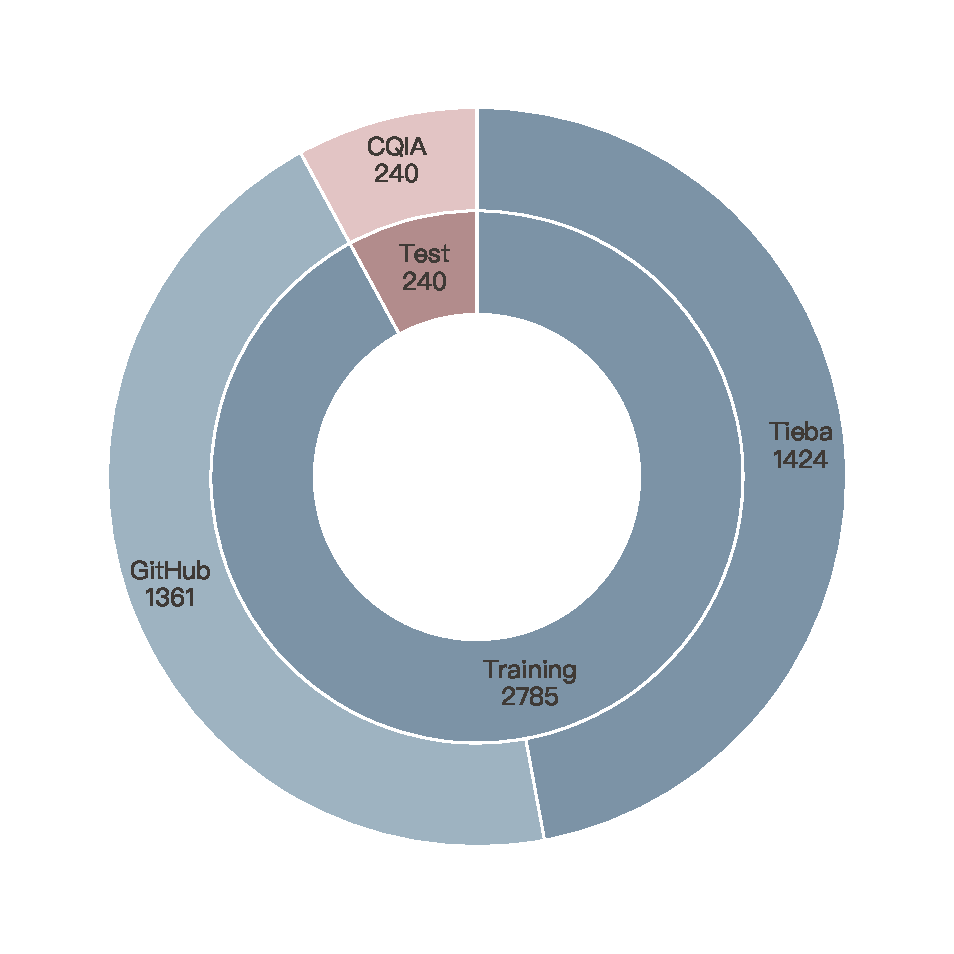
\includegraphics[width=0.5\textwidth]{dataset_source_donut.pdf}
    \caption{Source distribution of the data used in this report. The inner ring separates training from held-out test usage, while the outer ring shows the major source groups. Counts are displayed directly so the balance between the training mixture and the CQIA test set is easy to read.}
    \label{fig:dataset_donut}
\end{figure}

\begin{figure*}[t]
\centering
\resizebox{0.95\textwidth}{!}{%
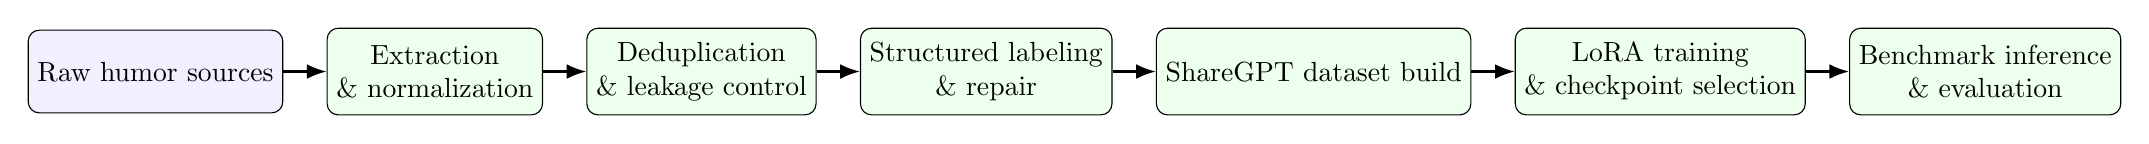
\begin{tikzpicture}[
    node distance=0.9cm and 0.55cm,
    box/.style={draw, rounded corners, align=center, minimum width=2.4cm, minimum height=1.05cm, fill=blue!6},
    stage/.style={draw, rounded corners, align=center, minimum width=2.65cm, minimum height=1.1cm, fill=green!7},
    arrow/.style={-{Latex[length=2.5mm]}, thick}
]
\node[box] (src1) {Raw humor sources};
\node[stage, right=of src1] (extract) {Extraction \\\& normalization};
\node[stage, right=of extract] (dedup) {Deduplication \\\& leakage control};
\node[stage, right=of dedup] (classify) {Structured labeling \\\& repair};
\node[stage, right=of classify] (build) {ShareGPT dataset build};
\node[stage, right=of build] (train) {LoRA training \\\& checkpoint selection};
\node[stage, right=of train] (eval) {Benchmark inference \\\& evaluation};

\draw[arrow] (src1) -- (extract);
\draw[arrow] (extract) -- (dedup);
\draw[arrow] (dedup) -- (classify);
\draw[arrow] (classify) -- (build);
\draw[arrow] (build) -- (train);
\draw[arrow] (train) -- (eval);
\end{tikzpicture}
}
\caption{Project workflow. Source texts are collected from benchmark and forum-style humor corpora, normalized into a consistent format, deduplicated to reduce leakage risk, labeled into the target JSON schema, and converted into ShareGPT-style SFT data. LoRA models are then trained under different rank and dataset-scope settings and evaluated on the CQIA benchmark with structured-output metrics and qualitative analysis.}
\label{fig:pipeline}
\end{figure*}

\section{Training Setup}
\subsection{Base Model and Fine-Tuning Configuration}
 \texttt{Qwen3-4B-Instruct-2507}~\cite{Yang2025Qwen3} is chosen as the base model and LoRA~\cite{Hu2021LoRA} is applied to all linear layers. Two LoRA ranks were tested: 8 and 16. To keep the scaling ratio stable, LoRA alpha was set to 16 for rank 8 and 32 for rank 16. Training used bf16 precision, cosine learning-rate decay with 10\% warmup, maximum sequence length 2048, and AdamW-style optimization inside the LoRA training stack.

The experiment contains four groups: rank 8 and rank 16 on the full dataset, and the same two ranks on the recent \texttt{last3} subset. Each configuration was trained for seven epochs, with checkpoints saved by epoch for later comparison.

\subsection{Hardware and Execution}
Training was run on an NVIDIA H800 GPU with 80 GB memory. The codebase is organized as a stage-wise pipeline under \texttt{scripts/}, with dedicated subdirectories for crawling, data processing, training, inference, and visualization. The minimal submission package in \texttt{upload/} keeps the reproducible path while excluding debug-only scripts.

The training and evaluation flow is simple: build the ShareGPT data, launch LoRA jobs with \texttt{run\_training.sh}, merge checkpoints with \texttt{batch\_merge.sh}, run vLLM-based inference~\cite{Kwon2023}, and compute metrics and charts with \texttt{eval\_metrics.py}. This keeps the submission reproducible without exposing the full development history.

\subsection{Example Prompts and Desired Outputs}
The target behavior can be illustrated with three short examples.
\begin{itemize}[leftmargin=1.5em]
    \item Prompt: \textit{咖啡严格来说是不是也可以叫豆浆？} Desired top-1 label: \textit{Wordplay}. The output should explain the literal decomposition of ``bean'' and ``liquid'' and return a ranked top-3 list.
    \item Prompt: \textit{石油也是油，为啥没人用它来炒菜？} Desired top-1 label: \textit{Strange Questions}. The output should identify the polysemy of ``oil'' and explain the false analogy.
    \item Prompt: \textit{失踪是不是丢人的事情？} Desired top-1 label: \textit{Wordplay}. The output should connect the joke to lexical decomposition and still remain valid JSON.
\end{itemize}

For the third example, a minimal target output can be written as follows:
\begin{lstlisting}[language=json]
{
    "thought_process": "The joke decomposes '失踪' by linking the morpheme '丢' to '丢人', creating a deliberate semantic misreading.",
    "top3_categories": [
        {"rank": 1, "category": "文字游戏", "confidence_score": 0.78, "reason": "Primary humor comes from lexical decomposition and semantic shift."},
        {"rank": 2, "category": "奇怪提问", "confidence_score": 0.15, "reason": "The sentence is phrased as a seemingly serious question built on a false premise."},
        {"rank": 3, "category": "地狱笑话", "confidence_score": 0.07, "reason": "A weak dark-humor interpretation is still possible because the topic involves disappearance."}
    ]
}
\end{lstlisting}

\section{Training and Evaluation Results}

\subsection{Evaluation Metrics}

For a test set of $N$ samples, let $y_i$ denote the gold top-1 category, let $\hat{y}_i$ denote the parsed prediction, let $S_i^{(3)}$ denote the predicted top-3 set, let $J_i$ indicate strict JSON validity, and let $R_i$ indicate parse success after tolerant extraction or repair. The main metrics are
\[
\mathrm{StrictAcc}=\frac{1}{N}\sum_{i=1}^{N}\mathbf{1}[J_i=1 \land \hat{y}_i=y_i],
\]
\[
\mathrm{Top1Acc}=\frac{1}{N}\sum_{i=1}^{N}\mathbf{1}[\hat{y}_i=y_i], \qquad
\mathrm{Top3Hit}=\frac{1}{N}\sum_{i=1}^{N}\mathbf{1}[y_i \in S_i^{(3)}],
\]
\[
\mathrm{JSONStrict}=\frac{1}{N}\sum_{i=1}^{N}\mathbf{1}[J_i=1], \qquad
\mathrm{VSR}=\frac{1}{N}\sum_{i=1}^{N}\mathbf{1}[R_i=1].
\]

\subsection{Loss Curves}

Figure~\ref{fig:training_loss_curve} shows that training loss decreases smoothly over 581 steps for the full-data runs and 217 steps for the recent-only runs, which suggests stable optimization under the LoRA setup. Validation loss reaches its minimum at step 400 for the full-data rank-16 run ($0.8859$) and then rises slightly, which points to mild overfitting. Figure~\ref{fig:strict_acc_curve} shows the held-out strict-accuracy trend on the CQIA benchmark. The full-data settings stay ahead of their recent-only counterparts, and the rank-16 run peaks at epoch 5 before flattening slightly.

Both rank settings on the full dataset converge well, but their late-epoch behavior differs slightly.

Rank 16 reaches the lowest validation loss at epoch 5 ($0.8859$) and then rises slightly, which suggests early overfitting. Rank 8 decreases more gradually and stays stable later in training. The gap is not large, but the pattern fits the intuition that a larger adapter learns the task faster and becomes more sensitive to over-training.

\begin{figure}[H]
    \centering
    \begin{minipage}[t]{0.48\textwidth}
        \centering
        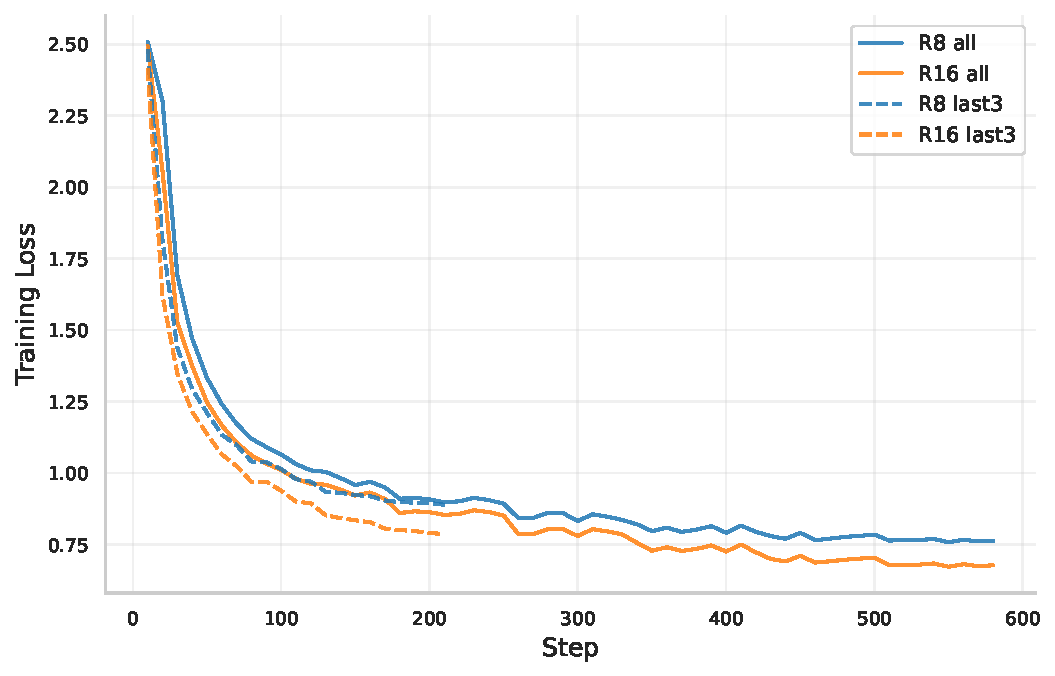
\includegraphics[width=\textwidth]{line_training_loss.pdf}
        \subcaption{Step-level training loss across the four experiment groups.}
        \label{fig:training_loss_curve}
    \end{minipage}\hfill
    \begin{minipage}[t]{0.48\textwidth}
        \centering
        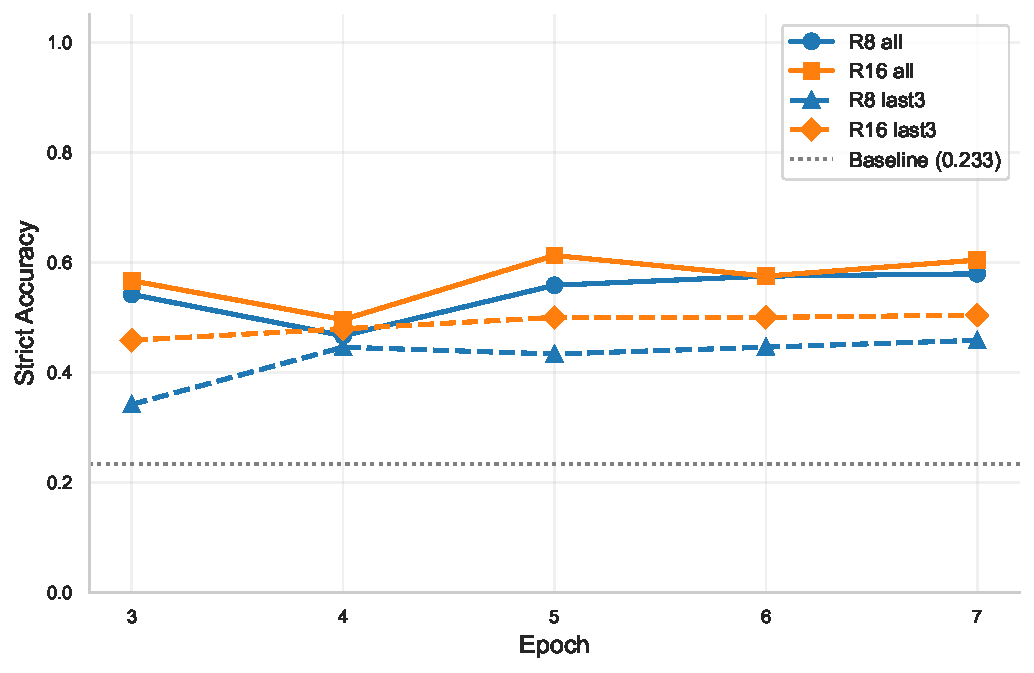
\includegraphics[width=\textwidth]{line_strict_accuracy.pdf}
        \subcaption{Held-out strict accuracy across epochs for the four experiment groups.}
        \label{fig:strict_acc_curve}
    \end{minipage}
    \caption{Training dynamics and downstream checkpoint quality. Training loss decreases smoothly in all four runs, while downstream strict accuracy peaks earlier for the full-data rank-16 setting than for the smaller recent-only subsets.}
\end{figure}



\begin{table}[H]
\centering
\small
\caption{Main before-versus-after metrics on the 240-sample CQIA test set.}
\label{tab:main_results}
\begin{tabular}{lcccc}
\toprule
Model & Strict Acc. & Top-1 Acc. & Top-3 Hit & JSON Strict \\
\midrule
Baseline & 0.233 & 0.233 & 0.588 & 0.996 \\
R8, epoch 7 & 0.579 & 0.579 & 0.871 & 0.996 \\
R16, epoch 5 & \textbf{0.613} & \textbf{0.613} & 0.883 & \textbf{1.000} \\
R16, epoch 7 & 0.604 & 0.604 & \textbf{0.892} & 1.000 \\
\bottomrule
\end{tabular}
\end{table}

\subsection{Quantitative Results}

Table~\ref{tab:main_results} summarizes the baseline and representative fine-tuned checkpoints. The baseline already produces mostly parseable JSON, but its actual label quality is weak. The best model, \texttt{r16\_e5}, improves top-1 accuracy from $0.233$ to $0.613$ and top-3 hit rate from $0.588$ to $0.883$ while maintaining a perfect valid-sample rate.

Across all 21 evaluated models, three patterns are clear. Full-data training beats the recent-only subset on every matched rank comparison. Rank 16 usually performs better than rank 8, although the gap is modest on the full dataset. Validation loss is also a useful checkpoint-selection signal: the lowest validation loss matches the highest downstream strict accuracy.

\begin{figure}[H]
    \centering
    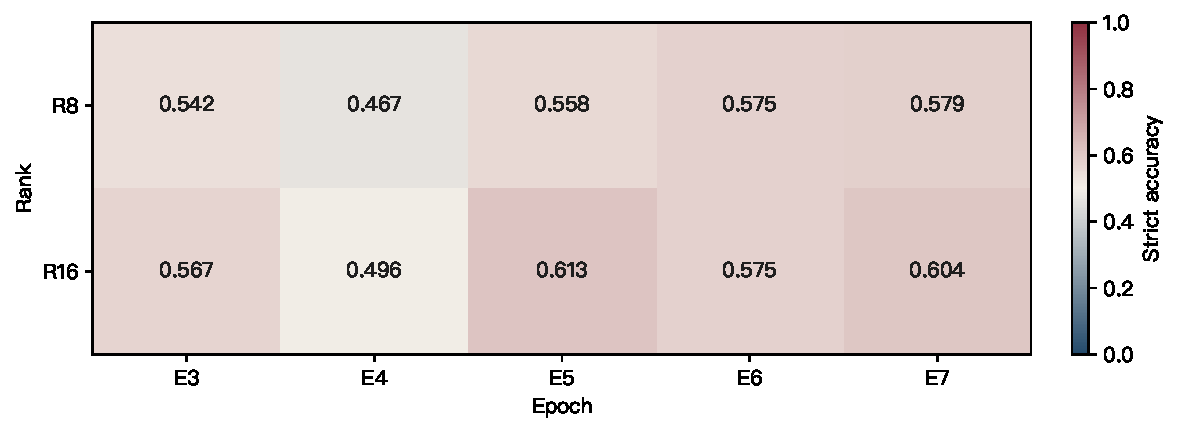
\includegraphics[width=0.82\textwidth]{heatmap_all_strict_accuracy.pdf}
    \caption{Strict-accuracy heatmap for the full-data experiments. Darker cells indicate stronger checkpoints, with the best result at rank 16, epoch 5.}
    \label{fig:heatmap_strict}
\end{figure}

\begin{figure}[H]
    \centering
    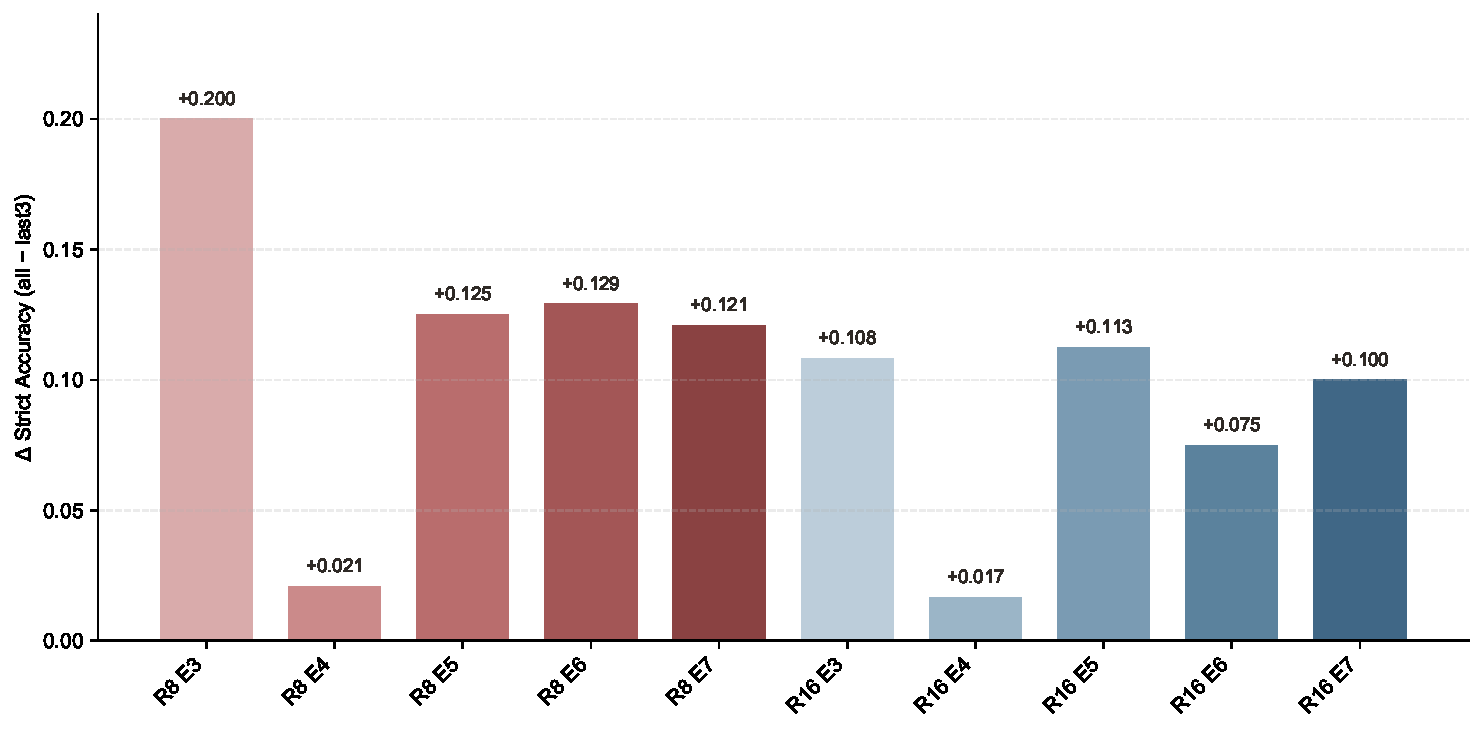
\includegraphics[width=0.82\textwidth]{bar_all_vs_last3_delta.pdf}
    \caption{Strict-accuracy advantage of full-data training over the \texttt{last3} subset. All bars are positive, showing that data volume matters more than recency in this task.}
    \label{fig:all_vs_last3}
\end{figure}

\subsection{Qualitative Results}
The qualitative comparison shows the same pattern. The base model often returns fluent but weakly grounded category lists. After SFT, the model follows the target schema more reliably and aligns better with the humor taxonomy.

Table~\ref{tab:qualitative_cases} summarizes five held-out examples used for qualitative analysis. Two improvements stand out. First, SFT reduces label confusion for \textit{Strange Questions}, a category that dominates the test set and that the baseline often misreads as dark humor or pseudo-scientific logic. Second, the post-SFT outputs match the structured-output target much more consistently: they include ranked predictions, explicit confidence scores, and reason fields with near-perfect validity.

\begin{table}[H]
\centering
\small
\caption{Representative before-versus-after cases on the CQIA test set.}
\label{tab:qualitative_cases}
\begin{tabularx}{\textwidth}{>{\raggedright\arraybackslash}p{0.3\textwidth} >{\raggedright\arraybackslash}p{0.12\textwidth} >{\raggedright\arraybackslash}p{0.12\textwidth} X}
\toprule
Prompt & Baseline Top-1 & SFT Top-1 & Observation \\
\midrule
苦行僧以苦为乐，那么他受苦是不是可以说他在奖励自己 & 弱智科学家 & 奇怪提问 & Baseline leans too hard on pseudo-reasoning; SFT catches the odd-question framing. \\
为什么医院床位那么紧张，不弄成上下铺呢？ & 地狱笑话 & 奇怪提问 & SFT fixes the context-driven misclassification and focuses on the naive false solution. \\
为什么白天能看见月亮，晚上却看不见太阳呢？ & 奇怪提问 & 奇怪提问 & Both are correct, but SFT adds ranked predictions and a cleaner schema. \\
失踪是不是丢人的事情？ & 文字游戏 & 文字游戏 & Both recognize the lexical joke; SFT makes the semantic decomposition more explicit. \\
并非无人爱我，病危通知单是死神小姐予我的情书 & 文字游戏 & 文字游戏 & Both miss \textit{Literary Absurdity}, which suggests remaining confusion between poetic style and lexical play. \\
\bottomrule
\end{tabularx}
\end{table}

Another representative prompt is ``天下没有不散的筵席，那么我们相聚的意义又是什么'', whose gold top-1 label is \textit{Literary Absurdity}. In the baseline output, the analysis is already fluent and the top-1 label is correct, but the \texttt{top3\_categories} field is only a plain string list. In the SFT output, the same prediction is rewritten into the target schema with explicit \texttt{rank}, \texttt{confidence\_score}, and \texttt{reason} fields for each candidate category, so the format finally matches the task definition.

\paragraph{Baseline output (sample 3).}
\begin{lstlisting}[style=promptstyle]
{
    "thought_process": "这个段子表面看似哲思，实则在‘天下没有不散的筵席’这一经典俗语基础上，提出一个荒诞的反问：既然聚会终将散场，那相聚的意义何在？...属于典型的‘文艺弱智’...",
    "top3_categories": [
        "文艺弱智",
        "奇怪提问",
        "人生态度"
    ]
}
\end{lstlisting}

\paragraph{SFT output (sample 3).}
\begin{lstlisting}[style=promptstyle]
{
    "thought_process": "这句话的核心结构是：先引用一句经典俗语‘天下没有不散的筵席’，然后顺着这个前提进行逻辑推演...语言优美且有哲理感，符合【文艺弱智】的特征...",
    "top3_categories": [
        {
            "rank": 1,
            "category": "文艺弱智",
            "confidence_score": 0.65,
            "reason": "语言具有哲理性和诗意感...完美契合‘兼具诗意与荒诞’的特征。"
        },
        {
            "rank": 2,
            "category": "古典弱智",
            "confidence_score": 0.2,
            "reason": "整句话构成了一个看似深刻的循环论证...利用了概念的偷换和语义漏洞。"
        },
        {
            "rank": 3,
            "category": "奇怪提问",
            "confidence_score": 0.15,
            "reason": "以疑问句形式呈现...符合‘看似合理实则利用认知盲区’的特征。"
        }
    ]
}
\end{lstlisting}

\begin{figure}[H]
    \centering
    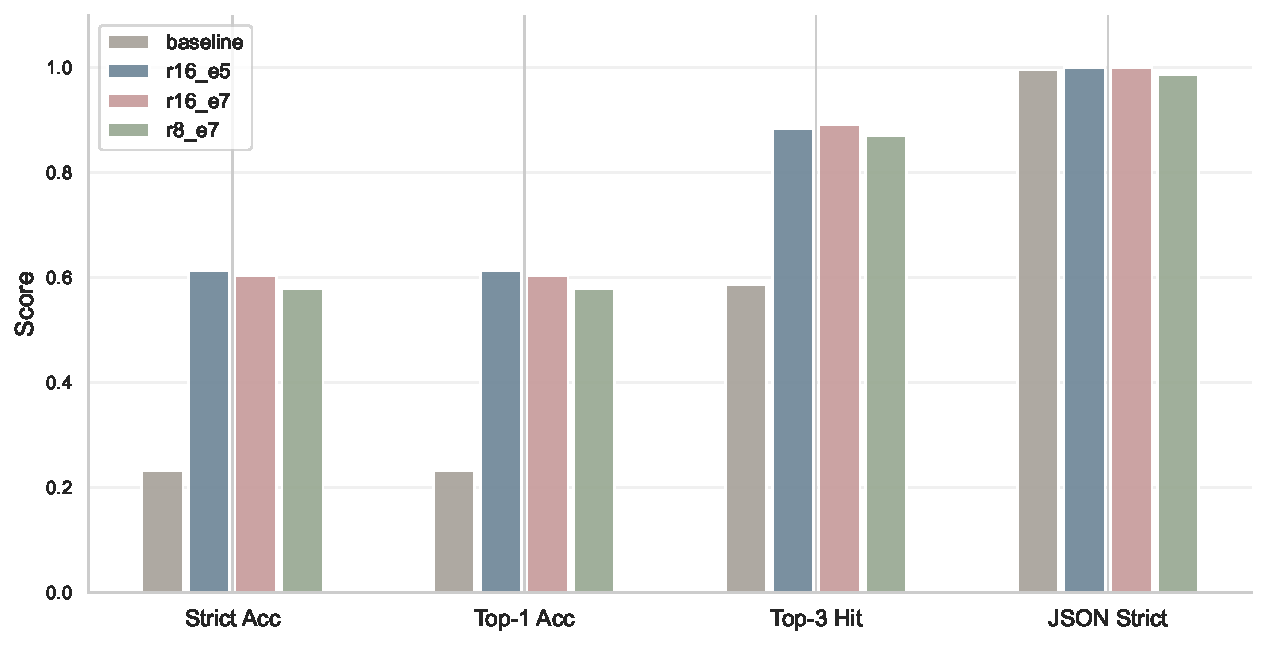
\includegraphics[width=0.82\textwidth]{bar_baseline_vs_top3.pdf}
    \caption{Comparison between the baseline and the top-performing fine-tuned checkpoints. The largest gains appear in strict accuracy and top-1 accuracy.}
    \label{fig:baseline_vs_top3}
\end{figure}

\section{Discussion and Conclusion}

This report presents a complete LoRA fine-tuning pipeline for structured Chinese humor classification using the Ruozhiba dataset, turning raw corpora into a clearly defined supervised fine-tuning target. The main result is simple: LoRA improves task performance substantially over the base instruct model, which means explicit structured supervision matters much more here than prompt-only control. The best configuration, rank 16 at epoch 5 on the full dataset, raises strict accuracy from 0.233 to 0.613 and the top-3 hit rate from 0.588 to 0.883 while maintaining a perfect valid-sample rate.

This improvement comes mainly from explicit task framing rather than from the base model's general fluency. A large part of that was the dataset rewriting process: category definitions, teacher-generated rationales, and ShareGPT formatting made the target much less underspecified. The comparison between the full dataset and the recent-only subset also suggests that this humor-classification task is data-hungry. Broader historical coverage helps more than restricting training to newer posts.

The gains are real, but some difficult categories still lag behind, especially \textit{Dark Humor}, \textit{Homophone Puns}, and \textit{Literary Absurdity}. Error analysis suggests that the model still struggles with fine distinctions, especially when it has to separate poetic absurdity from ordinary wordplay. The most obvious next step is targeted data augmentation together with clearer annotation guidelines for these edge cases.

\bibliographystyle{unsrt}
\bibliography{references}

\clearpage
\renewcommand{\thesection}{Appendix \Roman{section}}
\setcounter{section}{0}

\section{Expected JSON Output Schema}
\label{app:json_schema}

The expected response format follows the prompting and evaluation pipeline. A compact example is shown below.

\begin{lstlisting}[language=json]
{
    "thought_process": "Briefly explain the humor mechanism and why the ranked labels fit.",
    "top3_categories": [
        {
            "rank": 1,
            "category": "文字游戏",
            "confidence_score": 0.85,
            "reason": "Primary humor comes from lexical reinterpretation."
        },
        {
            "rank": 2,
            "category": "奇怪提问",
            "confidence_score": 0.10,
            "reason": "The utterance also resembles a naive but structured question."
        },
        {
            "rank": 3,
            "category": "弱智科学家",
            "confidence_score": 0.05,
            "reason": "A weak pseudo-rational framing remains possible."
        }
    ]
}
\end{lstlisting}

\section{Prompt Templates for Labeling and Inference}

The main category-definition table has already been provided in the body of the report. For completeness, the prompting style used for annotation and inference is summarized below.

\subsection*{Labeling-oriented prompt excerpt}
\begin{lstlisting}[style=promptstyle]
你是一个精通中文互联网亚文化、语言学和幽默解构的“弱智吧”资深吧友兼大模型文本分类评估专家。
请对输入的“弱智吧”风格言论进行深度分析，并选出最贴合该言论特征的 Top 3 类别。
请严格以 JSON 格式输出 thought_process 和 top3_categories。

可选类别：古典弱智、奇怪提问、弱智科学家、人生态度、文字游戏、地狱笑话、谐音梗、文艺弱智。
\end{lstlisting}

\subsection*{Inference-time system prompt excerpt}
\begin{lstlisting}[style=promptstyle]
你是一个弱智吧幽默解构专家。请对用户输入的段子进行深度分析，识别其幽默机制，
并输出 Top-3 分类结果。请以 JSON 格式输出，包含 thought_process 和
top3_categories 两个字段。

可选类别：古典弱智、奇怪提问、弱智科学家、人生态度、文字游戏、地狱笑话、谐音梗、文艺弱智。
\end{lstlisting}

\section{Additional Visualization Panels}

This appendix collects several supporting figures that were generated by the evaluation scripts but not placed in the main body. They provide a fuller view of optimization behavior, checkpoint selection, and class-level error structure without interrupting the central narrative of the report.

\begin{figure}[H]
    \centering
    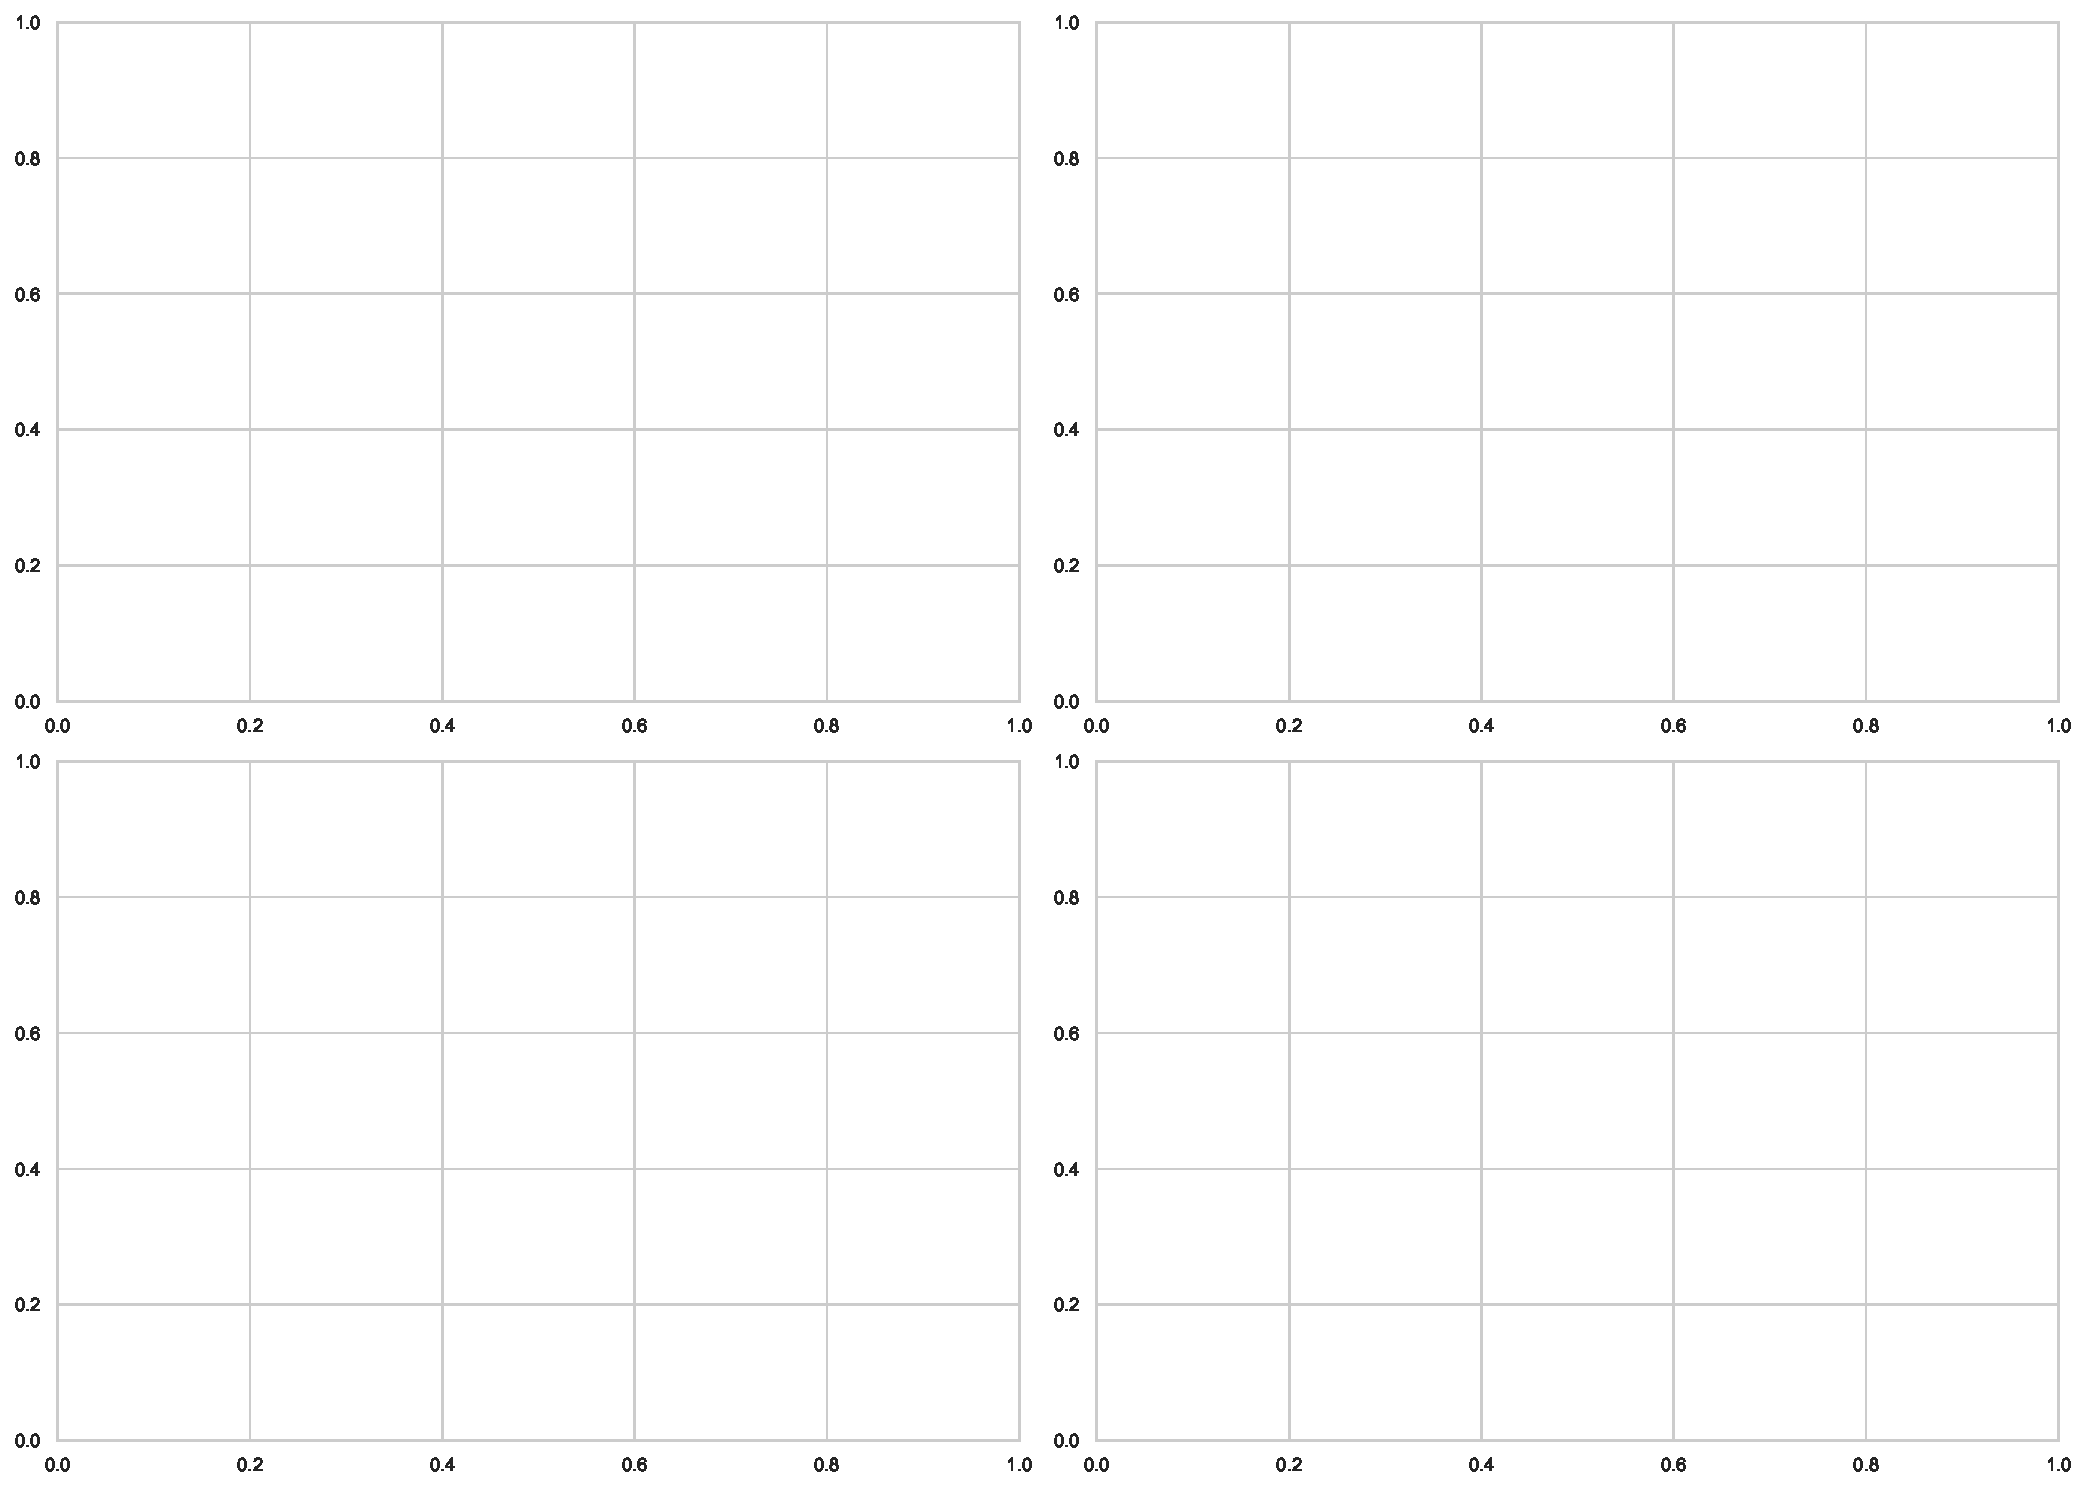
\includegraphics[width=0.88\textwidth]{grid_train_eval_loss.pdf}
    \caption{Train-loss and validation-loss curves for the four experimental groups. The full-data rank-16 configuration reaches a lower validation-loss minimum earlier than the others, while the recent-only subsets converge with fewer steps and a narrower improvement range.}
    \label{fig:grid_train_eval_loss_appendix}
\end{figure}

\begin{figure}[H]
    \centering
    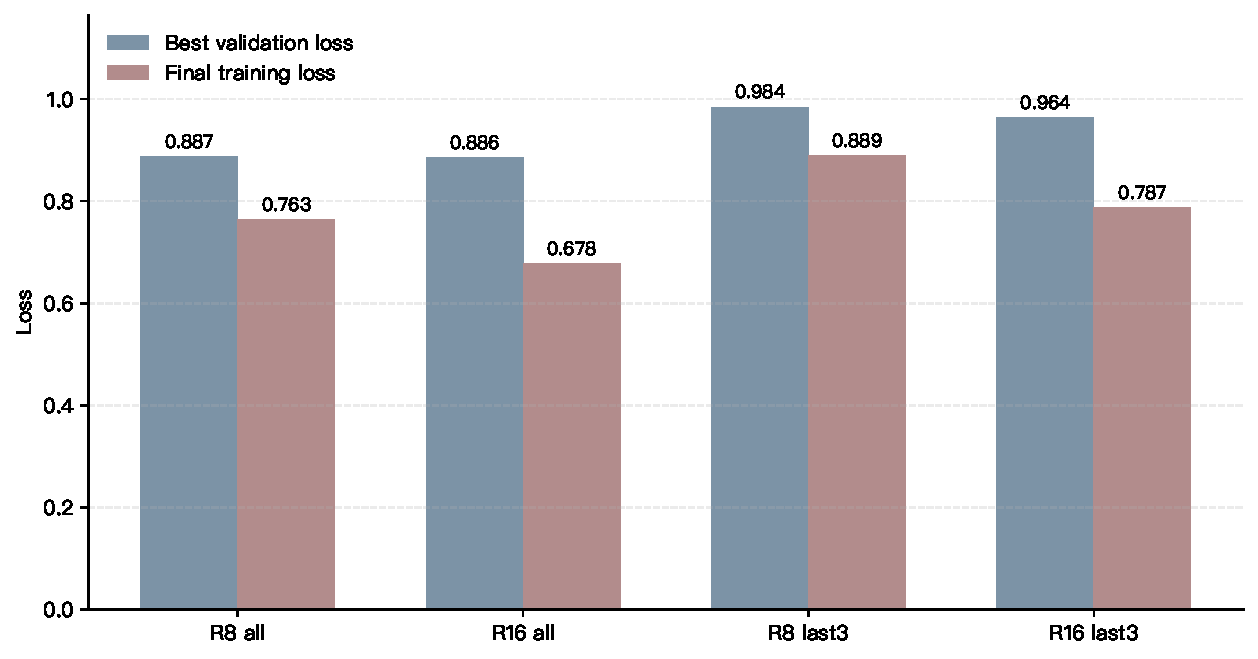
\includegraphics[width=0.74\textwidth]{bar_training_vs_validation_loss.pdf}
    \caption{Best validation loss versus final training loss for each training group. The gap is modest in all settings, but it is most visible for the full-data rank-16 run, which is consistent with the mild overfitting signal discussed in the main text.}
    \label{fig:bar_train_val_loss_appendix}
\end{figure}

\begin{figure}[H]
    \centering
    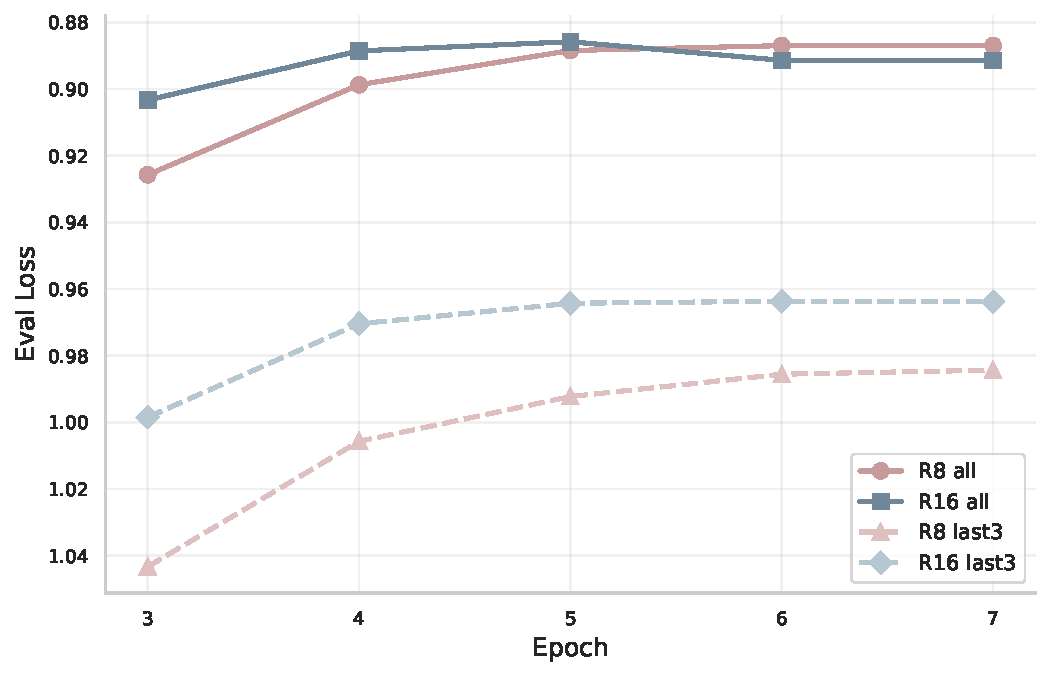
\includegraphics[width=0.74\textwidth]{line_eval_loss.pdf}
    \caption{Validation-loss trajectories across epochs. Lower values indicate better checkpoint quality, and the full-data settings remain more competitive than their \texttt{last3} counterparts throughout the training schedule.}
    \label{fig:line_eval_loss_appendix}
\end{figure}

\begin{figure}[H]
    \centering
    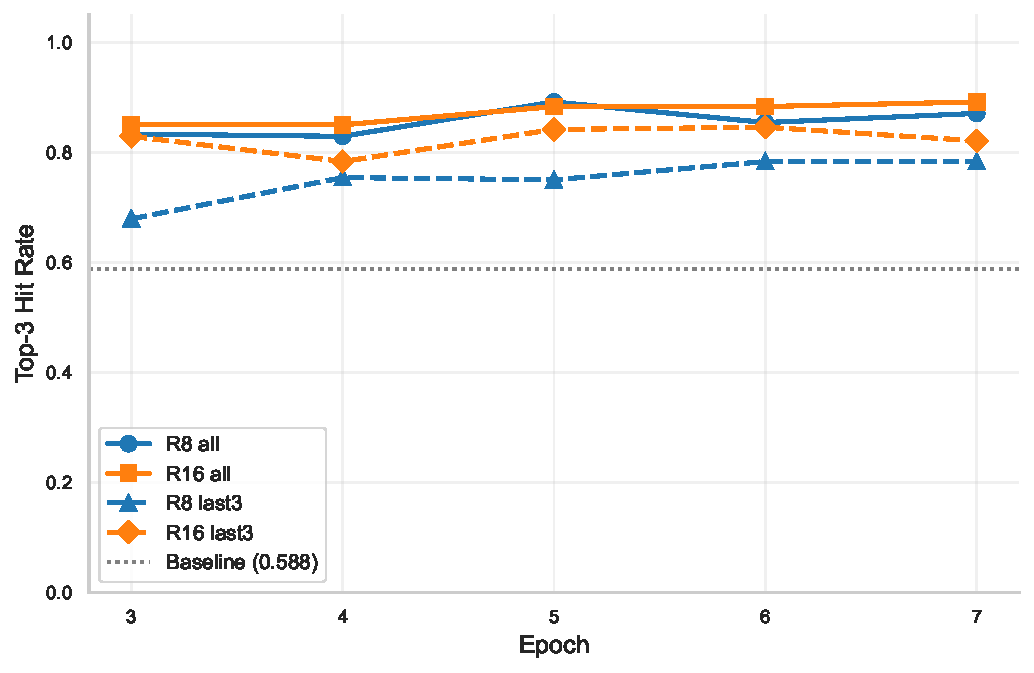
\includegraphics[width=0.74\textwidth]{line_top3_hit_rate.pdf}
    \caption{Top-3 hit rate across epochs. Even when the top-1 prediction is not perfect, the full-data checkpoints usually retain the correct label within their ranked candidate set.}
    \label{fig:line_top3_hit_rate_appendix}
\end{figure}

\begin{figure}[H]
    \centering
    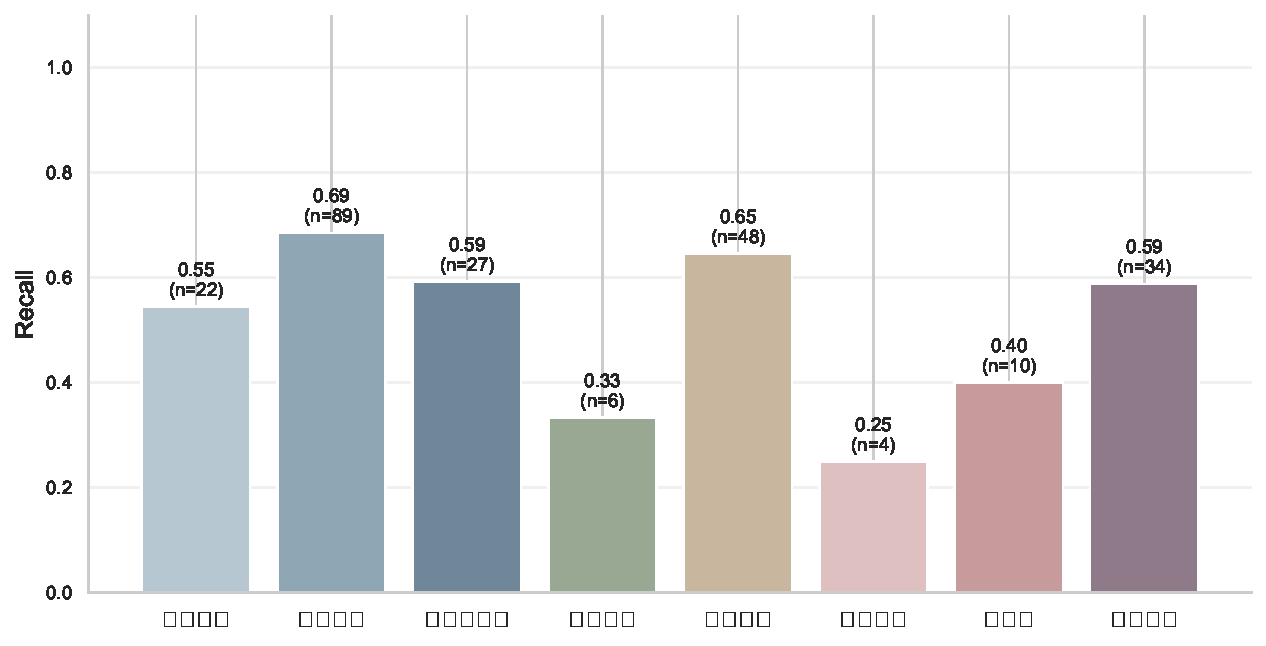
\includegraphics[width=0.78\textwidth]{bar_per_category_recall_r16_e5.pdf}
    \caption{Per-category recall for the best-performing checkpoint \texttt{r16\_e5}. Performance is strongest on frequent categories such as \textit{Strange Questions}, while rarer classes remain more difficult.}
    \label{fig:bar_per_category_appendix}
\end{figure}

\begin{figure}[H]
    \centering
    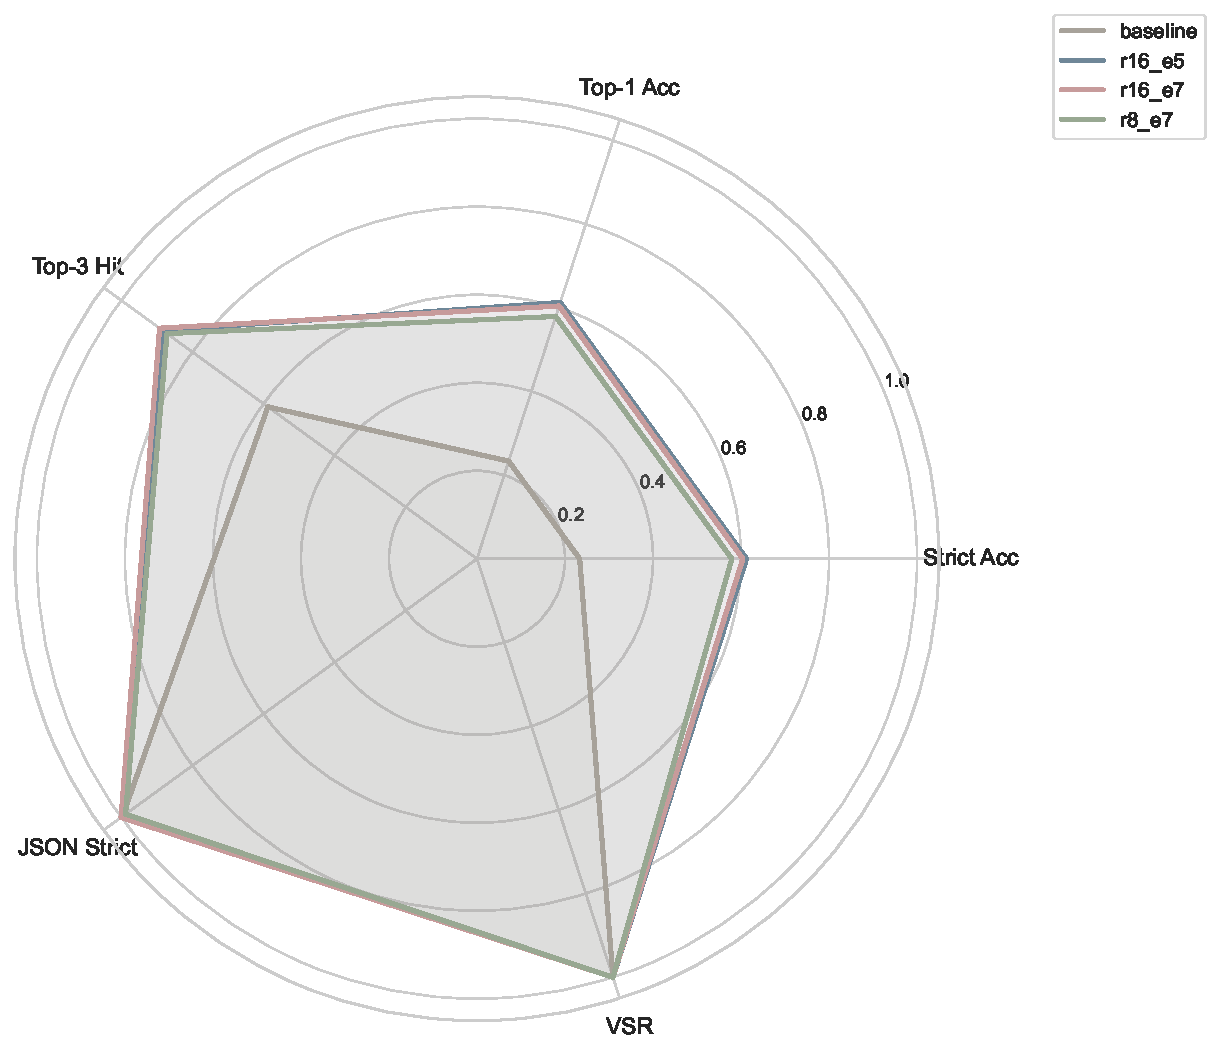
\includegraphics[width=0.72\textwidth]{radar_top_models.pdf}
    \caption{Radar comparison of the baseline and the top-performing fine-tuned checkpoints. The fine-tuned models dominate the baseline on structured-output reliability and classification accuracy simultaneously.}
    \label{fig:radar_top_models_appendix}
\end{figure}

\end{document}
